\documentclass[a4,center,fleqn]{NAR}
\usepackage{lipsum}
% Enter dates of publication
\copyrightyear{XXXX}
\pubdate{XX XXXX XXXX}
\pubyear{XXXX}
\jvolume{XX}
\jissue{XX}

\articlesubtype{This is a draft}

\begin{document}

\title{???}

\author{%
Rodrigo Vargas Honorato\,$^{1,2}$,
Jorge Roel Touris\,$^{1}$
Alexandre Bonvin\,$^1$%
\footnote{To whom correspondence should be addressed.
Tel: +44 000 0000000; Fax: +44 000 0000000; Email: xxx@yyyy.ac.zz}}

\address{%
$^{1}$Bijvoet Center for Biomolecular Research, Faculty of Science, Utrecht University, Utrecht 3584CH, the Netherlands
$^{2}$Brazilian Biosciences National Laboratory (LNBio), Brazilian Center for Research in Energy and Materials (CNPEM), Zip Code 13083-970, Campinas, Sao Paulo, Brazil.}
% Affiliation must include:
% Department name, institution name, full road and district address,
% state, Zip or postal code, country

\history{%
Received XXXX X, XXXX;
Revised XXXX X, XXXX;
Accepted XXXX X, XXXX}

\maketitle

\begin{abstract}
blablabla
\end{abstract}


\section{Introduction}

Computational modeling of protein structures, interactions and dynamics has been advancing steadily in the past decades. Nonetheless researchers still face challenges when modeling large biomolecular systems with. Reducing the representation level from all-atom to coarse-grained is a way to bypass limitations such as algorithmic efficiency and available computing power \cite{Vendruscolo2011}.

The main objective of a coarse-grained representation is to reduce the degrees of freedom, replacing amino acids (either fragments or entire side chains) with pseudo-atoms. The first coarse-grained protein models were built in the 70's and were successfully able to simulate an entire folding process \cite{Levitt1975}. Further development of the model accounted for the variable orientation of the pseudo sidechains and torsional potential for the main chain degrees of freedom were based on the statistical analysis of conformational properties of dipeptides \cite{Levitt1976}. 

Since proteins adopt a well-defined three-dimensional arrangement defined by both the conformational restraints of the main-chain as well as interactions with the environment by the side chains, it is expected that a coarse-grained representation of a protein contains all its crucial elements. The main objective of this representation is to reduce the number of degrees of freedom inherent to a protein structure. 

% How this can be used for docking

The development of coarse-grained force fields have taken two directions; physics-based, following the same philosophy of it full-atom counterpart, basing it on molecular physics and knowledge-based that takes advantage the growing databases via statistical analysis. Here we apply the knowledge-based forcefield CG MARTINI \cite{Marrink2007} which has been extended to account for nucleic-acids <ref>, in our data-driven docking program HADDOCK <ref>. Whilst there are some CG docking algorithms for protein-protein <ref attract, pydockcg, haddock> the approach has nos been applied protein-DNA before.

We demonstrate this feature by modeling the polycomb repressive complex 1 (PRC1) in complex with its nucleosome core particle substrate. PRC1 is assembled as a multi-component arrangement which is responsible for chromatin structure remodeling both directly and through the establishment and removal of histone post-translational modifications [10.1038/nature13890].

% **************************************************************
% Keep this command to avoid text of first page running into the
% first page footnotes
\enlargethispage{-65.1pt}
% **************************************************************


\section{MATERIALS AND METHODS}

\subsection{Forcefield implementation}


\section{MARTINI DNA Extension}

The MARTINI CG DNA model was systematically parametrized according to the MARTINI philosophy, being backwards compatible with all other MARTINI model implementations. Experimental values such as liquid densities and partitioning free energies of small solutes between polar and nonpolar solvents are used to determine non-bonded interaction parameters\cite{Uusitalo2015}.

As previously described, four non-hydrogen atoms are mapped to one CG bead which describes one or more chemical building blocks along with its properties. The parametrization used by Uusitalo and collaborators combines top-down (experimental data) and bottom-up (atomistic simulations) methodologies to parametrize the CG DNA model. The CG bead types for each nucleobase were selected based on partition free energies from water to chloroform or hydrated octanol. Bonded interactions have been fitted to reproduce dihedral, angle and bond distributions from atomistic simulation of short single stranded DNAs (ssDNAs). For double stranded DNA (dsDNA) an elastic network was devised to maintain the double helical structure.

Here each nucleotide is mapped to six or seven CG beads. The phosphate accounts for one bead and sugar for two, pyrimidines are represented as three-bead rings and purines as four-bead rings (Figure \ref{fig:dnacg}). After changing the representation of dsDNA bases the resulting distance between them are 0.34 nm, which lead to issues in the CG model. To account for that, a smaller bead size was created for the CG DNA model with $\sigma = 0.32nm$ (68\% smaller than the regular CG bead) and named T, for tiny. 

%\begin{figure}
%	\centering
%	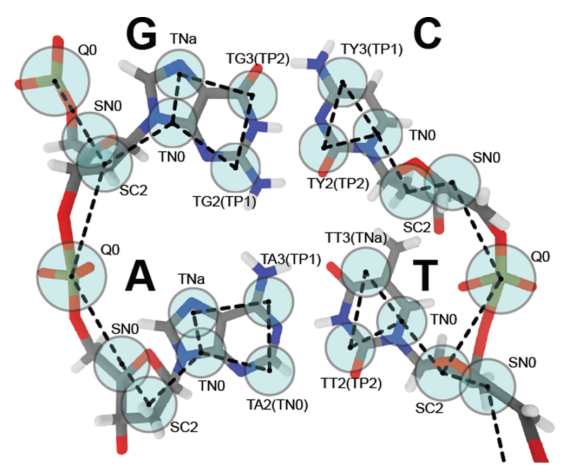
\includegraphics[width=0.7\linewidth]{dna_cg}
%	\caption{DNA backbone is modeled with one bead describing the phosphate and two beads describing the sugar. The pyrimidines are modeled with three beads and the purines with four beads. T-prefix marks the beads that use the new tiny bead type. For hydrogen bonding beads, the new special bead types are shown together with the bead type describing their interactions with all beads except the special hydrogen bonding beads (in parentheses) \cite{Uusitalo2015}.}
%	\label{fig:dnacg}
%\end{figure}

Hydrogen bonding between bases is a crucial factor for the formation of dsDNA and since the standard MARTINI model does not describe the directional hydrogen bonds, the interaction between hydrogen bonding beads was tweaked. Interactions are defined in a pairwise fashion for each bead type, henceforth eight special beads were added for the purpose of replicating this crucial bond.


\begin{align}
\mathrm{LD}^r = \frac{\mathrm{LD}}{A_\mathrm{iso}}
= 1.5 S \left( 3 \cos^2 \alpha_i - 1 \right)
\end{align}


\subsection{Materials subsection two}
\lipsum

\begin{equation*}
\mathrm{LD} \left( t \right) =
\sum\limits_i
a_i \exp \left( \frac{-t}{\tau_i} \right)
\end{equation*}


\begin{figure}[t]
\begin{center}
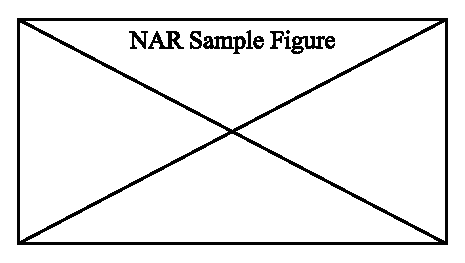
\includegraphics{NAR-fig1.eps}
\end{center}
\caption{Caption for figure within column.}
\label{NAR-fig1}
\end{figure}


\section{RESULTS}

\subsection{Benchmark}
\lipsum

\subsection{Revisiting T95}
\lipsum


\begin{figure*}[t]
\begin{center}
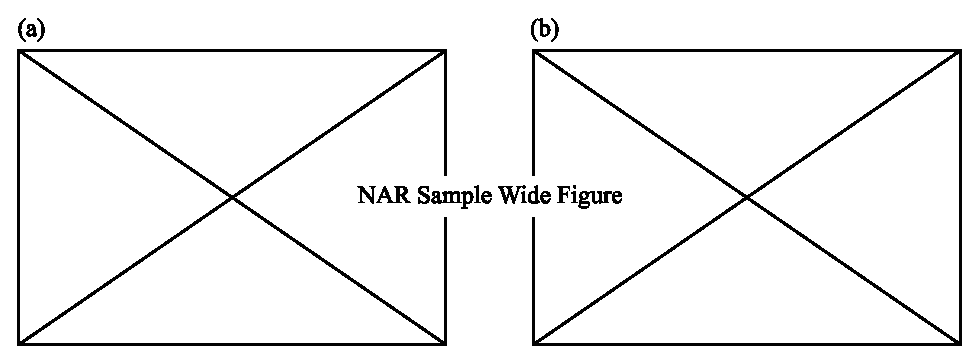
\includegraphics{NAR-fig2.eps}
\end{center}
\caption{Caption for wide figure over two columns.
\textbf{(a)} Left figure.
\textbf{(b)} Right figure (see (a)).
}
\label{NAR-fig2}
\end{figure*}

\section{DISCUSSION}

\subsection{Discussion subsection one}
\lipsum

\subsection{Discussion subsection two}
\lipsum

\section{CONCLUSION}
\lipsum

\section{ACKNOWLEDGEMENTS}

Text. Text. Text. Text. Text. Text. Text. Text. Text. Text. Text.
Text. Text. Text. Text.


\subsubsection{Conflict of interest statement.} None declared.
\newpage


\begin{thebibliography}{4}

% Format for article
\bibitem{1}
Author,A.B. and Author,C. (1992)
Article title.
\textit{Abbreviated Journal Name}, \textbf{5}, 300--330.

% Format for book
\bibitem{2}
Author,D., Author,E.F. and Author,G. (1995)
\textit{Book Title}.
Publisher Name, Publisher Address.

% Format for chapter in book
\bibitem{3}
Author,H. and Author,I. (2005)
Chapter title.
In
Editor,A. and Editor,B. (eds),
\textit{Book Title},
Publisher Name, Publisher Address,
pp.\ 60--80.

% Another article
\bibitem{4}
Author,Y. and Author,Z. (2002)
Article title.
\textit{Abbreviated Journal Name}, \textbf{53}, 500--520.

\end{thebibliography}

\end{document}
